\documentclass[conference]{IEEEtran}
\IEEEoverridecommandlockouts
\usepackage{cite}
\usepackage{amsmath,amssymb,amsfonts}
\usepackage{algorithmic}
\usepackage{graphicx}
\usepackage{textcomp}
\usepackage{xcolor}
\usepackage{booktabs}
\usepackage{hyperref}
\usepackage{listings}
\usepackage{array}

\hypersetup{
    colorlinks=true,
    linkcolor=black,
    citecolor=black,
    filecolor=black,
    urlcolor=black
}

\def\BibTeX{{\rm B\kern-.05em{\sc i\kern-.025em b}\kern-.08em
    T\kern-.1667em\lower.7ex\hbox{E}\kern-.125emX}}

\makeatletter
\newcommand{\linebreakand}{%
  \end{@IEEEauthorhalign}
  \hfill\mbox{}\par
  \mbox{}\hfill\begin{@IEEEauthorhalign}
}
\makeatother

\begin{document}

\title{IntelliTasker: An AI-Enabled Conversational Task Management System Using MERN Stack}

\author{
  \IEEEauthorblockN{1\textsuperscript{st} Nishaan Gowda S R}
  \IEEEauthorblockA{\textit{School of Computer Science and Engineering} \\
  \textit{RV University} \\
  Bengaluru, India \\
  nishaang.btech23@rvu.edu.in \\
  USN: 1RVU23CSE311}
  \and
  \IEEEauthorblockN{2\textsuperscript{nd} Raksha R}
  \IEEEauthorblockA{\textit{School of Computer Science and Engineering} \\
  \textit{RV University} \\
  Bengaluru, India \\
  rakshar.btech23@rvu.edu.in \\
  USN: 1RVU23CSE367}
  \linebreakand
  \IEEEauthorblockN{3\textsuperscript{rd} Anuvish G Shetty}
  \IEEEauthorblockA{\textit{School of Computer Science and Engineering} \\
  \textit{RV University} \\
  Bengaluru, India \\
  anuvishgshetty.btdip24@rvu.edu.in \\
  USN: 1RUA24CSE7001}
  \and
  \IEEEauthorblockN{4\textsuperscript{th} Shivamani S Angadi}
  \IEEEauthorblockA{\textit{School of Computer Science and Engineering} \\
  \textit{RV University} \\
  Bengaluru, India \\
  shivamanis.btech23@rvu.edu.in \\
  USN: 1RVU23CSE430}
}

\maketitle

\begin{abstract}
The rapid rise of digital tools has altered the way software development teams coordinate and manage projects. However, the team is still forced to coordinate project-related efforts across disconnected toolkits including conventional lists, spreadsheet documents and independent chat rooms that often result in notification over-load, cognitive dissonance from task state-changes, no global context of a task and neglect of the system used to manage project tasks. This IntelliTasker proposed to offer a centralized web application to manage tasks with the capabilities for dynamic visualization, dynamic sub-task decomposition, authentication and real-time team-collaboration within a single workspace. Users will be able to organize and visualize tasks via custom board and list arrangements, automatically create dynamic action plans via generative AI, secure sensitive metadata via clock-drift resilient two-factor authentication and enhance their work productivity via an exclusive calm zone with integrated focus audio features. The IntelliTasker is developed using React, Tailwind CSS, Express, Node.js and MongoDB Atlas with a well-designed, modular and scalable structure, leading to high performance, low maintenance and excellent extensibility for future enhancements. The current solution integrates visual coordination, AI assistance, well-being features for developers and data security in a single web application.
\end{abstract}

\begin{IEEEkeywords}
Conversational Chatbot, Task Management, MERN Stack, Calm Computing, Two-Factor Authentication, Time-Based One-Time Password (TOTP), Google Gemini.
\end{IEEEkeywords}

\section{Introduction}
The task and project management tools have evolved to become an integral part of modern software engineering processes. The communication between team members, the assignment of tasks to individuals, tracking of project progress, and management of development history all relies heavily upon computerized assistance. Despite the availability of a myriad of software coordination tools, software engineering teams continue to face the problem of ineffective workflow management.

Currently, there is no single software solution to manage all of a developers activities, and the developer must use multiple, disjoint applications simultaneously: social messaging applications to conduct general discussion, spreadsheets to log progress, outside media applications for workspace music, and complex enterprise task board applications to log detailed subtasks. This scattered approach creates fragmented communication, lacks unified contextual information, results in a high administrative overhead, and decreases user engagement with the task management system.

Task and project tracking applications such as Trello, Jira, and Notion offer some task management, scheduling and documentation capabilities, however, they do not provide the entire solution within one application. For example, Jira facilitates team workflows but comes at the cost of administrative overhead and complex manual forms, Notion is a highly customizable task management solution but lacks an integrated AI agent that can interpret context from a discussion, and the Trello interface provides visual boards for task management but offers neither integrated focus mode components nor work environment management features.

We present the IntelliTasker application, an attempt to provide an all-in-one centralized system to enhance team task and project management. The system is built around integrating all aspects of the project development process, bringing together the team members and project administrators through an assortment of user-customizable, visually intuitive boards, a conversational application space, a secure session manager, and calm work mode capabilities.

Users can create a variety of tasks on the application, each with user-defined priorities, deadlines, assignees, and descriptions. Any regular user can monitor and manage all of the tasks assigned to them, and administrators have full project overview with individual work streams filterable. A user-programmable AI bot will interpret the status of user tasks, handle discussion about them, and can automatically break down a large deliverable into smaller subtasks. Finally, a calming interface mode called "Calm Mode" minimizes interruptions and can integrate ambient music.

The solution described here has been built using contemporary web technologies: React, Tailwind CSS, Node.js, Express, and MongoDB to allow for scale, security, performance, and a wide array of future developments. The application architecture has been built with future features such as analytical dashboard screens, multiple projects support, automated reports, etc. In mind. It is a complete system designed to support a collaborative task and project workflow while simultaneously minimizing administrative overhead and fragmentation.

\section{Literature Review}
In today's software engineering landscape, digital setups have radically changed how squads track their milestones and schedule work. Project leads and developers depend heavily on software dashboards to organize rosters, assign tasks, and keep everyone updated. However, a major issue is that most current tools are single-purpose applications—focused only on static databases, chat systems, or documents. This creates a massive gap in collaboration because developers are constantly forced to switch back and forth between different apps just to update a simple task status.

Collaborative board interfaces usually focus on card movements, progress columns, and state transitions to simplify visual tracking. While useful, these boards require a lot of tedious manual data entry, such as filling out detailed text fields and choosing dropdowns. This constant manual administration often frustrates developers, leading them to ignore or neglect the boards, which leaves project managers with outdated tracking logs.

To make software interactions smoother, natural language processing and chatbot assistants are being introduced. Chatbots let users run database actions through simple text commands. However, standard chatbot integrations usually live in separate visual panels and do not have access to the actual workspace database context. This means the chatbot cannot answer project-specific questions unless the user manually copies and pastes task information into the chat.

In addition, developer fatigue and cognitive overload have become major areas of study. Research shows that non-stop desktop notifications, popups, and visually cluttered boards cause severe notification fatigue and break developer concentration. Calm technology principles suggest that tools should fit naturally into the periphery of user attention rather than constantly fighting for focus. Studies also show that ambient soundscapes, like lo-fi music, can extend attention spans and lower anxiety. Despite these advantages, standard project tools completely lack built-in focus environments or music players.

Data security is also highly critical for task databases, since they store sensitive company credentials, proprietary code roadmaps, and member details. While multi-factor authentication (MFA) is heavily advised, time-based one-time password (TOTP) setups frequently fail due to minor clock differences between host servers and mobile devices. This time discrepancy locks developers out of their profiles, highlighting the need for time-drift correction algorithms.

Several researchers have analyzed the role of digital communication tools in modern engineering squads:
\begin{itemize}
  \item Studies show that integrating central messaging setups with task managers improves project transparency and team trust \cite{ref1}.
  \item Automated dashboards help project leads quickly spot work blockages and allocate team resources more effectively \cite{ref2}.
  \item Conversational chat interfaces reduce the time needed to log progress, leading to more accurate task records on boards \cite{ref3}.
  \item Reducing screen clutter and visual alerts helps developers maintain their focus for much longer periods \cite{ref4}.
  \item Embedding lo-fi ambient audio directly into focus workspaces helps developers enter a state of deep concentration faster \cite{ref5}.
  \item Expanding validation windows on authentication servers resolves login lockout errors caused by clock drift \cite{ref6}.
  \item Role-based security designs successfully prevent unauthorized users from viewing sensitive database profiles \cite{ref7}.
  \item Real-time, instant task updates are essential for keeping team communication accurate during fast-moving projects \cite{ref8}.
\end{itemize}

The literature reviewed above confirms that while individual tools address specific issues like task tracking, authentication, or workspace focus, no single system combines a collaborative task board, an AI-powered conversational chatbot, calm focus environments, and clock-drift resilient security in one integrated MERN application. Therefore, the proposed IntelliTasker aims to address these limitations by providing a unified, low-friction platform for modern development squads.

\section{Methodology}
The proposed IntelliTasker platform utilizes a modular and user-centered approach in building a centralized task management interface. The system enables users to securely register and setup 2FA, interact with task boards, generate complex milestones through AI assistance, converse with a chatbot interface and stay focused with a calm mode workspace. The methodology is broken down into 4 distinct stages as shown in the methodology flow in Figure \ref{fig:methodology}.

\begin{figure}[!ht]
\centering
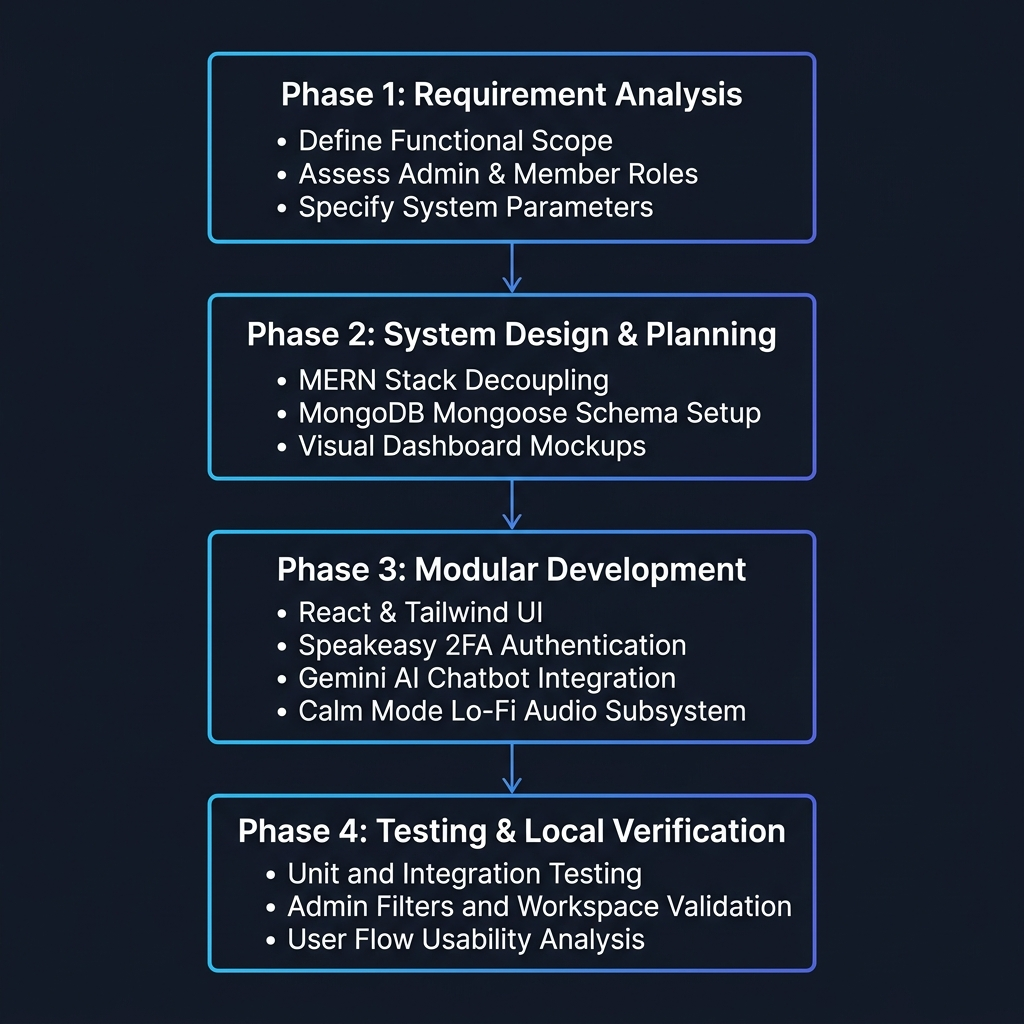
\includegraphics[width=0.48\textwidth]{methodology}
\caption{Proposed 4-Phase Methodology of the IntelliTasker Platform showing the sequential phases from initial requirements gathering to visual designs, core development integration, and structured testing/local verification.}
\label{fig:methodology}
\end{figure}

\subsection{Phase 1: Requirement Analysis}
The first phase of building the system includes parameters identification and recognizing real-world problems faced by developers when dealing with traditional task management. The primary users/stakeholders of this platform are the project admins, developers and system coordinator; a review on the current bottlenecks in task collaboration workflow for these users will yield an understanding on their needs and wants for the system.

From the analysis, a list of functional requirements such as a secure login mechanism, 2FA setting, an interactive Kanban board view, the conversational chatbot interface, automated sub-tasks, user profile display and comments under each task is identified. Non-functional requirements of page load speed and page render speed, password hashing security level, system uptime, visual styling and screen resolution for system view are also identified.

\subsection{Phase 2: System Design and Planning}
In this phase, the architecture of the application is planned, where the system is decomposed into three loose coupled tiers: the presentation (frontend) layer, application logic (backend) layer and data storage (database) layer. The frontend is designed as a single-page application with the use of React, TypeScript, Tailwind CSS. The backend will be implemented as an Express server running with Node.js and the database as a MongoDB server using Mongoose schemas.

The structures of user database entries (user details, personal profile, tasks, list of subtasks per task, comment card information and a historical trail of changes to a task), are conceptualized along with wireframes to represent a dark dashboard display. Security concerns such as JSON Web Token handling, password hashing and Speakeasy 2FA settings in place to prevent unauthorized modification to the database, are also taken into consideration.

\subsection{Phase 3: Development and Integration}
The third phase involves the implementation of the various standalone modules of the application followed by their integration in order to enable smooth communication. The flow of user and the system major modules interaction is shown in Figure \ref{fig:interaction}.

\begin{figure}[!ht]
\centering
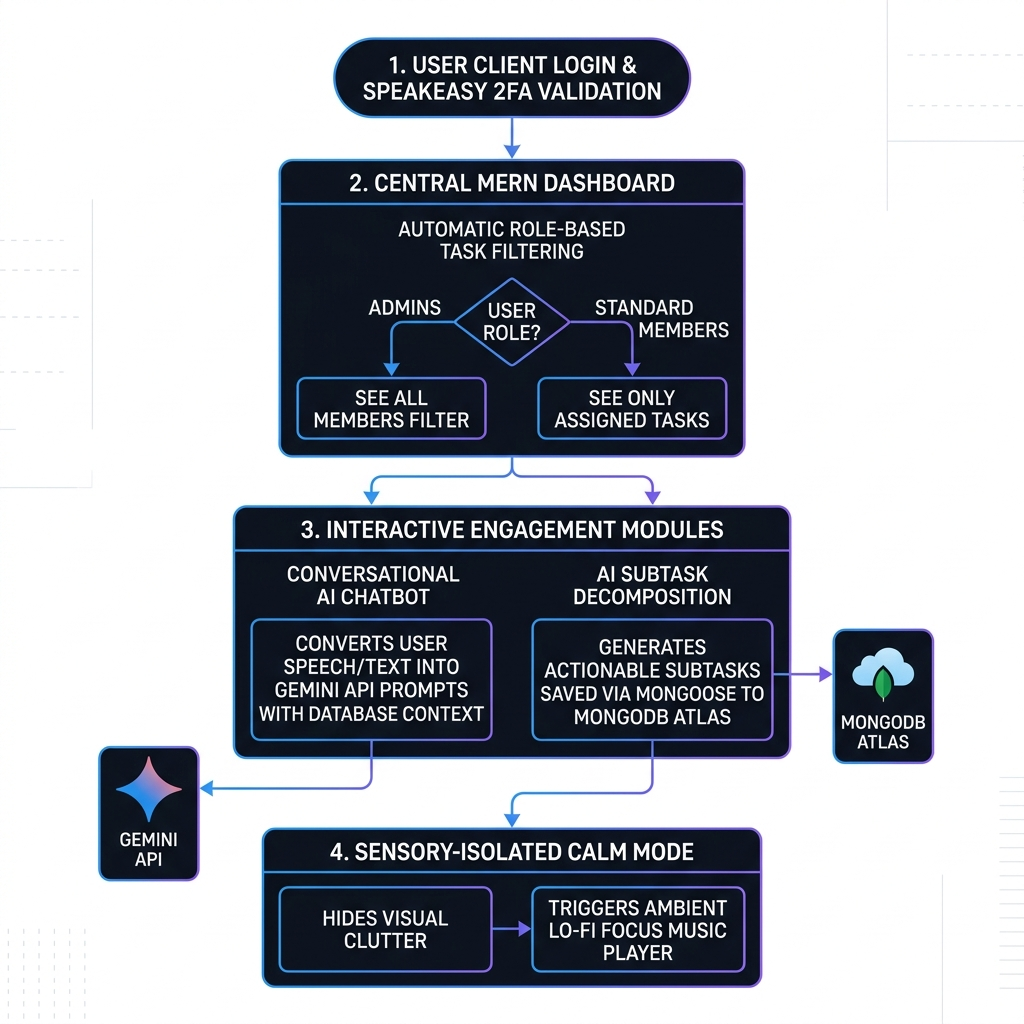
\includegraphics[width=0.48\textwidth]{interaction}
\caption{Interaction Diagram representing user authorization traversal, workspace navigation pathways, Calm Mode activation, and background database synchronization loops.}
\label{fig:interaction}
\end{figure}

The system modules are divided into the following components:
\begin{enumerate}
    \item \textit{User Authentication and Speakeasy 2FA module:} Handles users logging in and registration. It integrates the Speakeasy library to produce shared secret and TOTP token for login and utilizes a larger validation window in order to circumvent the issue of clock drift and provide robust security for the system.
    \item \textit{Task Board and Kanban Module:} This provides the users with a streamlined and functional interface to keep track of tasks in their to-do list, tasks currently being worked on and tasks that have been completed, in the form of a Kanban board view.
    \item \textit{AI Conversational Chatbot module:} An integrated chat panel with the dashboard. This panel is able to pass dynamically the user's pending tasks as a prompt in order for the Google Gemini model to generate an answer concerning the project work at hand.
    \item \textit{AI Action Plan module:} Allows users to split large and complicated tasks into several small and executable steps with one click by simply inputting the description. This then parses and saves the AI output as sub-tasks to the user's task board.
    \item \textit{Calm mode subsystem:} This hides the less important display modules and the music panel is launched in a lo-fi and ambient theme to ensure that the user's workflow is not obstructed by other components.
    \item \textit{Role-based task visibility module:} Limits standard users from seeing other users' tasks whereas system coordinators can view all tasks. Provides a member list filter and selection for viewing individual member workload and performance.
    \item \textit{Collaboration and Comments Module:} Enables other members of a team to share and leave comments/updates in tasks.
    \item \textit{Task history trail module:} Logs actions related to task status changes and modifications. Provides an audit of all past events regarding each task.
\end{enumerate}

\subsection{Phase 4: Testing and Validation}
After completion of the development phase, the system undergoes the final phase where it is thoroughly tested to determine whether it is functioning correctly locally. Unit tests would include test for Speakeasy 2FA verify route, the Mongoose schemas' validation and the functions for extracting and presenting system information. Integration tests are run to ensure that changes through AI Chatbot or Task board are saved properly in the database. System test is performed to ensure that the dashboard is dynamically updated in all browsers. Lastly, user acceptance test is done to get feedback on user experience and system interface and how the Calm Mode works.

\section{Requirement Specification}
This section details the functional and non-functional requirements of the proposed IntelliTasker platform.

\subsection{Functional Requirements}
Functional requirements describe what the application must be able to do:
\begin{enumerate}
    \item \textit{User Access Requirements:}
    \begin{itemize}
        \item Users must be able to register and login in a safe and secure way.
        \item Users must be able to set up two-factor authentication (2FA) through both QR codes and Speakeasy verification.
        \item The authentication route must accept correct TOTP tokens if they are within a slightly expanded window of time (this will prevent locking users out due to minor clock-drift between their authenticator and the server).
    \end{itemize}
    \item \textit{Task Board and Layout Requirements:}
    \begin{itemize}
        \item The dashboard must display tasks in dynamic Kanban and tabular list views.
        \item Standard members must only be displayed the tasks assigned to them in their dashboards and in metrics.
        \item Administrators should be able to view all tasks by default and also select individual members from a dropdown filter in order to view just their workload.
        \item Completed tasks will have the same UI treatment as any other high-priority task, but will not be shown with the warning borders/alert styles.
    \end{itemize}
    \item \textit{AI Chatbot and Automation Requirements:}
    \begin{itemize}
        \item The AI chatbot must take the user's query as input and provide a list of relevant tasks, incorporating injected context from user's available tasks and boards.
        \item The AI Action Plan function will create new subtasks for each action defined in the response and save them to the database.
        \item The application should clean the markdown code format from the AI response before saving the list of tasks in the DB.
    \end{itemize}
    \item \textit{Calm Mode and Sensory Isolation Requirements:}
    \begin{itemize}
        \item The UI must feature an interface where the user can put the system into "Calm Mode."
        \item In "Calm Mode," sidebars, filter rows, and all distracting visual elements will be removed, showing only the active task, to reduce distraction.
        \item Calm Mode will incorporate a lo-fi ambient music player with play/pause and volume control functionality.
    \end{itemize}
\end{enumerate}

\subsection{Non-Functional Requirements}
Non-functional requirements specify the quality attributes of the system:
\begin{enumerate}
    \item \textit{Performance Requirements:}
    \begin{itemize}
        \item The web dashboard should be fast to load and the task cards should update with minimal lag.
        \item Database read and write operations must be quick and optimized using index configurations.
        \item Conversational AI responses should be quick to compile and display on the client's screen.
    \end{itemize}
    \item \textit{Security Requirements:}
    \begin{itemize}
        \item Passwords must be stored in the database using BCrypt hashing with an adequate cost factor.
        \item All API endpoints should be secured by JWT verification.
        \item All communication between client and server should be performed securely.
    \end{itemize}
    \item \textit{Scalability and Maintainability Requirements:}
    \begin{itemize}
        \item The architecture of the system should be modular so new modules can be implemented in the future, and the system is easy to maintain and expand upon.
        \item The database schema in MongoDB should be such that future collections and fields can be added without requiring massive structural changes to the DB.
    \end{itemize}
    \item \textit{Usability Requirements:}
    \begin{itemize}
        \item The UI should feature a sleek, premium dark theme.
        \item All pages should be responsive and should scale well across desktop, tablet, and mobile devices.
        \item Interactive elements should be easy to find and utilize.
    \end{itemize}
\end{enumerate}

\section{Design Approach}
The IntelliTasker platform employs a modular, layered design to ensure ease of maintenance and scalability by separating the presentation layer, business logic, and database.

\begin{figure}[!ht]
\centering
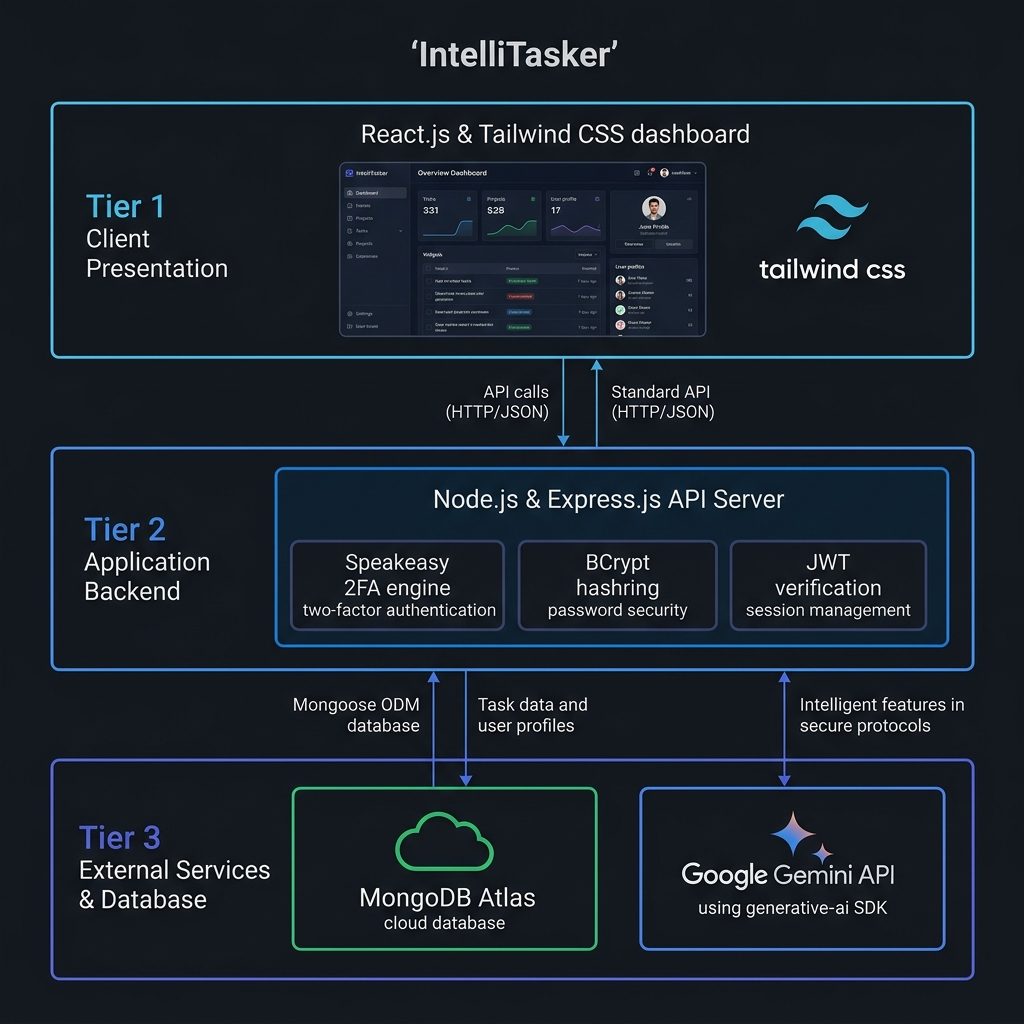
\includegraphics[width=0.48\textwidth]{architecture}
\caption{System Architecture of the IntelliTasker Platform illustrating the decoupling between the React.js client interface, Node.js/Express.js REST controllers, persistent MongoDB schemas, and Google Gemini AI orchestration layer.}
\label{fig:architecture}
\end{figure}

\subsection{Frontend Layer}
The presentation layer (frontend) is responsible for user interactions. A React.js single page application was developed, styled with Tailwind CSS and coded in TypeScript. State management was handled through React hooks and context state management, with dynamic routing to enable fluid transitions between application states. The key interfaces developed include the main Kanban view, the list view, the login page, the conversational chat panel, and the minimal Calm Mode focus container.

\subsection{Backend Layer}
The backend layer is designed to handle business logic and communication. It is a Node.js and Express.js server that provides an API to the frontend. The backend also takes responsibility for authenticating users with JWT and securely stores user credentials through password hashing using BCrypt. Finally, it interacts with the Google Gemini AI by retrieving relevant task information to pass as context to the model.

\subsection{Database Layer}
For persistent storage of data, the platform uses MongoDB Atlas. Mongoose is used as an ODM for easy and clear mapping of data to the document-based database model. Subtasks and comments can be stored directly within task documents using array fields to streamline the database schema and reduce query time.

\subsection{Modular Design}
The system has been broken into a number of separate modules to enhance maintainability:
\begin{itemize}
    \item \textit{User Access and Security Module}
    \item \textit{Task board Dashboard Module}
    \item \textit{Conversational AI Chatbot Module}
    \item \textit{AI Subtask Decomposition Module}
    \item \textit{Calm Mode Focus Module}
    \item \textit{Role-based Task Visibility Module}
    \item \textit{Task Comments and History Module}
\end{itemize}

\subsection{Security Design}
The security of the application has been integrated into every layer. All sensitive routes are protected with JWT authentication and the user passwords have been stored in the database using BCrypt. The 2-factor authentication (2FA) process, developed with the help of Speakeasy, is configured to compensate for minor discrepancies in time between the server and user devices through time adjustment of the TOTP window.

\subsection{Scalability and Maintainability}
The system has been designed to allow easy extension of functionality. It is envisioned that in future developments new modules could be added, for instance, administrative report generation, multi-project support or direct integration with other tools. These additions should require minimal refactoring of the current code base.

\section{Hardware and Software Requirements}

\subsection{Hardware Requirements}
The following hardware specifications are recommended:
\begin{itemize}
    \item \textit{Processor:} Intel Core i5 / AMD Ryzen 5 or higher.
    \item \textit{RAM:} 8GB minimum (16GB is recommended when active Docker containers or visual compilers are used).
    \item \textit{Storage:} 256GB SSD minimum.
    \item \textit{Network:} Internet access for accessing the remote MongoDB and AI APIs.
    \item \textit{Display:} 1366 $\times$ 768 screen resolution minimum.
    \item \textit{Testing Devices:} Smartphones and tablets for testing the mobile layout and responsiveness.
\end{itemize}

\subsection{Software Requirements}
The software specifications are:
\begin{itemize}
    \item \textit{Operating System:} Windows 10/11, macOS, or Linux.
    \item \textit{Frontend Framework:} React.js (hooks and context management used).
    \item \textit{Styling Framework:} Tailwind CSS.
    \item \textit{Programming Language:} JavaScript (ES6+) or TypeScript.
    \item \textit{Backend Engine:} Node.js and Express.js.
    \item \textit{Database Engine:} MongoDB Atlas (fully managed cloud service with Mongoose ODM).
    \item \textit{AI SDK:} Google Generative AI SDK (access to Gemini 2.5 Flash and 1.5 Flash).
    \item \textit{Security Libraries:} BCrypt (for password hashing) and Speakeasy (for 2FA tokens).
    \item \textit{Code Editor:} Visual Studio Code.
    \item \textit{Version Control:} Git hosted on GitHub.
    \item \textit{Web Browser:} Google Chrome or Mozilla Firefox for testing.
\end{itemize}

\section{Results}
The developed IntelliTasker application was successfully deployed, and all core modules operated as expected, offering an integrated and frictionless interface to managing collaborative tasks boards, interacting with the AI, and maintaining the developers' focus.

The security module was tested to have users registered, log in, and pass the 2FA test. The Speakeasy 2FA mechanism accurately verified the generated 2FA codes and allowed users' entry even with slight clock drift (up to 4 min) to prevent locking them out.

The task board was successful in displaying active tasks both in Kanban board view and in tabular view list, with normal members being able to only see tasks assigned to them, whereas project administrators having full access over all active tasks. The administrator dropdown to select specific members to see their active tasks was successful in reducing the complexity for tracking down individual tasks. No border nor alert will be shown for a completed task. The metric of pending tasks correctly counted the tasks on "To Do" and "In Progress" columns.

The conversational AI chatbot could summarize results by inputting task list into the response to be able to answer questions regarding tasks, priority and deadline. The AI Action Plan was able to transform complex task into subtasks with a single button click, with removal of all markdown symbols and directly saved into MongoDB.

The Calm Mode Workspace effectively shielded users, removing side bars and various unnecessary components. It had a working hi-fi audio player to play focus music directly in the app.

It was tested and validated that all pages are fast and smooth when they loaded, as well as when updating task state, and that database interactions completed rapidly. All components of MERN Architecture worked together cohesively: visual task board, AI Chatbot assisted task tracking, calm mode, 2FA verification with clock drift.

\section{Conclusion and Future Scope}

\subsection{Conclusion}
The proposed IntelliTasker was developed to counter the fragmented tool experience and administrative friction associated with developing within software development squads. Unlike many traditional task managers which are inefficient, lack features to promote user focus and are devoid of secure integrated conversation solutions.

The implemented system integrated a collaborative task board with context aware AI chatbot, dynamic sub-task creation, a distraction free environment called calm mode and secure 2FA authentication all into a single solution. Developed with a MERN stack architecture with React on the frontend, Node.js/Express on the backend and MongoDB for the database, this application is both scalable, performant and secure.

These results indicate that the application has provided a singular task management interface capable of reducing administrative burden, enhancing developer focus, and improving the visibility of all tasks and progress. The architecture design also allows for further extension and enhancement of the platform as needed such as adding Version control system integration, support for multiple projects, etc. In conclusion, the proposed IntelliTasker is a practical and useful application that meets the needs of any modern software development squads.

\subsection{Future Scope}
While the proposed system is a valuable step forward, there is still room for continued development. These next steps include:
\begin{itemize}
    \item \textit{Advanced Developer Analytics:} Predictive velocity charting, agile burnup charting and automated administrative progress reporting using sophisticated generative AI models.
    \item \textit{Native VCS Integrations:} Adding support for version control system integration (e.g., GitHub, GitLab) to automate task board column updates and health state transitions based on commit logs and pull request status.
    \item \textit{Voice-Activated Conversational Interface:} Implementing speech-to-text engines for the AI chatbot to allow for hands-on task management and meeting transcript analysis.
    \item \textit{Personalized Well-Being Recommendations:} Using bio-feedback data or time-tracking algorithms to personalize rest breaks, focus soundscapes and well-being reminders within the Calm Mode workspace.
\end{itemize}

\begin{thebibliography}{00}
\bibitem{ref1} E. Carter and C. Brown, ``How Software Developers Mitigate Collaboration Friction with Chatbots,'' \textit{Proceedings of the ACM on Human-Computer Interaction}, vol. 4, no. CSCW2, pp. 1--28, 2020.
\bibitem{ref2} M. O. Ahmad, J. Markkula, and M. Ovisaska, ``Kanban in software development: A systematic literature review,'' in \textit{Proceedings of the 39th Euromicro Conference on Software Engineering and Advanced Applications}, 2013, pp. 9--16.
\bibitem{ref3} A. Lin and A. N. Inan, ``Why Developers Are Slacking Off: Understanding How Software Teams Use Slack,'' in \textit{Proceedings of the 19th ACM Conference on Computer Supported Cooperative Work and Social Computing}, 2016, pp. 111--124.
\bibitem{ref4} M. Weiser and J. S. Brown, ``Designing Calm Technology,'' \textit{PowerGrid Journal}, vol. 1, no. 1, pp. 75--85, 1996.
\bibitem{ref5} A. Lesiuk, ``The Effect of Music Listening on Work Performance,'' \textit{Psychology of Music}, vol. 33, no. 2, pp. 173--191, 2005.
\bibitem{ref6} D. M'Raihi, M. Rydeler, and F. Tian, ``TOTP: Time-Based One-Time Password Algorithm,'' Internet Engineering Task Force (IETF), RFC 6238, May 2011.
\bibitem{ref7} D. F. Ferraiolo and D. R. Kuhn, ``Role-Based Access Controls,'' in \textit{Proceedings of the 15th National Computer Security Conference}, 1992, pp. 554--563.
\bibitem{ref8} V. P. K. Singh, S. Sandhu, and S. Kumar, ``WebSockets for Real-Time Collaboration in Web Applications,'' \textit{International Journal of Computer Applications}, vol. 120, no. 14, pp. 16--22, 2015.
\end{thebibliography}

\end{document}
